\section*{Phụ lục}
\addcontentsline{toc}{section}{Phụ lục}
\section{Danh sách lược đồ use case}

\begin{figure}[H]
    \centering
    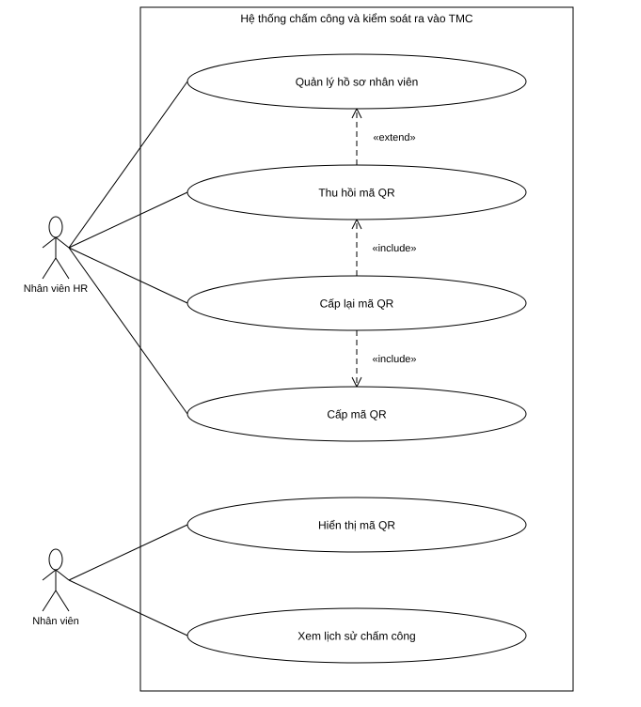
\includegraphics[width=\textwidth,height=0.72\textheight,keepaspectratio]{figures/appendix_use_case/uc_quan_ly_nguoi_dung_va_ma_qr.png}
    \caption{Sơ đồ use case nhóm Quản lý người dùng và mã QR}
    \label{fig:uc-quan-ly-nguoi-dung-ma-qr}
\end{figure}

\begin{figure}[H]
    \centering
    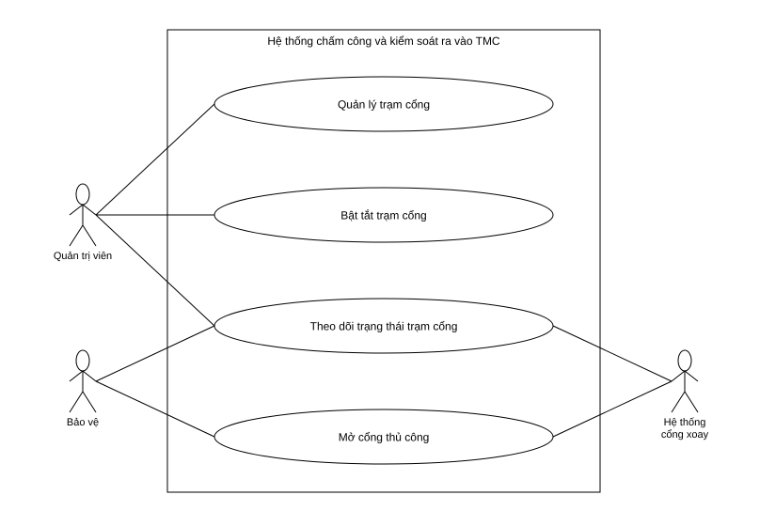
\includegraphics[width=\textwidth,height=0.72\textheight,keepaspectratio]{figures/appendix_use_case/uc_quan_ly_tram_cong.png}
    \caption{Sơ đồ use case nhóm Quản lý trạm cổng}
    \label{fig:uc-quan-ly-tram-cong}
\end{figure}

\begin{figure}[H]
    \centering
    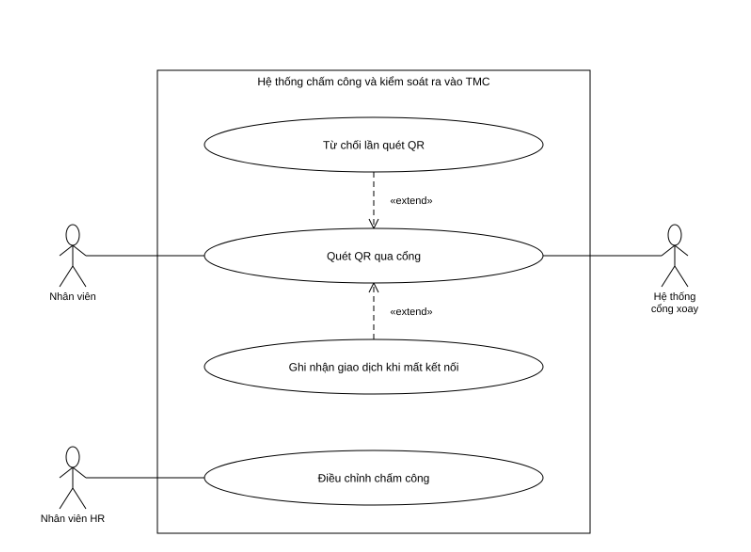
\includegraphics[width=\textwidth,height=0.72\textheight,keepaspectratio]{figures/appendix_use_case/uc_ghi_nhan_su_kien_cham_cong.png}
    \caption{Sơ đồ use case nhóm Ghi nhận sự kiện chấm công}
    \label{fig:uc-ghi-nhan-su-kien-cham-cong}
\end{figure}

\begin{figure}[H]
    \centering
    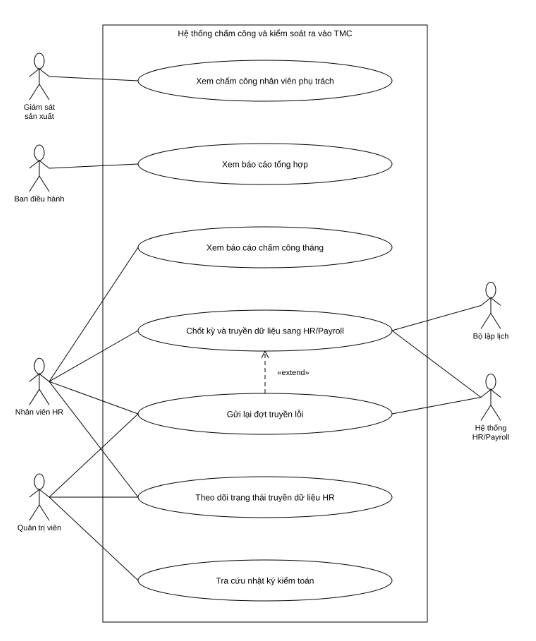
\includegraphics[width=\textwidth,height=0.72\textheight,keepaspectratio]{figures/appendix_use_case/uc_bao_cao_hr_payroll_kiem_toan.png}
    \caption{Sơ đồ use case nhóm Báo cáo, truyền dữ liệu HR/Payroll và kiểm toán}
    \label{fig:uc-bao-cao-hr-payroll-kiem-toan}
\end{figure}

\begin{figure}[H]
    \centering
    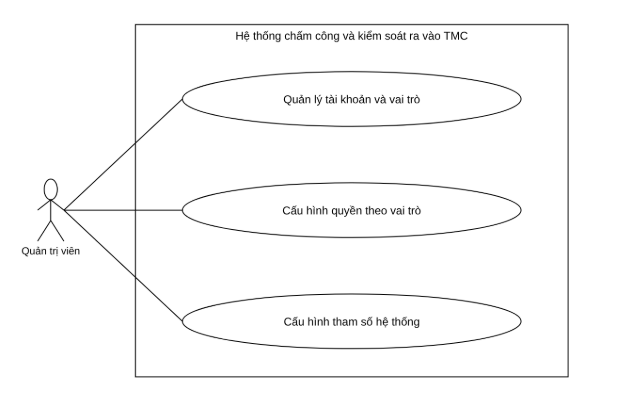
\includegraphics[width=\textwidth,height=0.72\textheight,keepaspectratio]{figures/appendix_use_case/uc_quan_tri_he_thong.png}
    \caption{Sơ đồ use case nhóm Quản trị hệ thống}
    \label{fig:uc-quan-tri-he-thong}
\end{figure}

\clearpage

\section{Use case quan trọng và đặc tả}

Nhóm chọn 4 use case có ý nghĩa kiến trúc trong số các use case ở phần thiết kế yêu cầu vì chúng gắn với các FR đánh dấu ASR. Bảng dưới đây liệt kê các use case được chọn và lý do lựa chọn; các phần tiếp theo đặc tả từng use case.

\small
\renewcommand{\arraystretch}{1.25}
\begin{longtable}{|>{\raggedright\arraybackslash}p{2.8cm}|>{\raggedright\arraybackslash}p{3.0cm}|>{\raggedright\arraybackslash}p{3.0cm}|>{\raggedright\arraybackslash}p{5.8cm}|}
\caption{Các use case có ý nghĩa kiến trúc} \\
\hline
\textbf{Use case} & \textbf{FR liên quan} & \textbf{Đặc tính kiến trúc} & \textbf{Lý do chọn} \\
\hline
\endfirsthead
\hline
\textbf{Use case} & \textbf{FR liên quan} & \textbf{Đặc tính kiến trúc} & \textbf{Lý do chọn} \\
\hline
\endhead
\hline
\multicolumn{4}{r}{\textit{Còn tiếp sang trang sau...}} \\
\hline
\endfoot
\hline
\endlastfoot
UC-01. Quét QR qua cổng & FR-08, FR-10, FR-11, FR-12, FR-13, FR-14, FR-15, FR-16, FR-17 & Performance, Availability, Data Integrity & Là luồng chính của hệ thống: phải xử lý nhanh, ghi nhận giao dịch chính xác và tiếp tục hoạt động khi mất kết nối. \\
\hline
UC-02. Thu hồi mã QR & FR-01, FR-02, FR-04, FR-05, FR-06, FR-23, FR-25 & Security, Availability & Hiệu lực thu hồi phải đến được các trạm cổng trong tối đa 60 giây (INV-02), nên ảnh hưởng cách phân phối dữ liệu QR xuống trạm. \\
\hline
UC-03. Điều chỉnh chấm công & FR-16, FR-18, FR-21, FR-22, FR-23, FR-25 & Data Integrity, Auditability & Giao dịch chấm công bất biến; điều chỉnh phải giữ bản gốc và để lại dấu vết (INV-06, INV-08). \\
\hline
UC-04. Chốt kỳ và truyền dữ liệu sang HR/Payroll & FR-21, FR-22, FR-23, FR-28 & Reliability, Interoperability & Dữ liệu phải có mặt ở HR/Payroll trước 12:00 ngày 1 (NFR-03); kỳ đã khóa chỉ nhận điều chỉnh qua đợt bổ sung (INV-09). \\
\end{longtable}
\normalsize

\subsection{UC-01. Quét QR qua cổng}

\noindent\textbf{Actor:} Nhân viên (chính); Hệ thống cổng xoay (phụ).

\noindent\textbf{Mô tả:} Nhân viên đưa mã QR vào máy quét tại trạm cổng để vào hoặc ra nhà máy. Hệ thống xác thực mã, mở cổng, ghi giao dịch chấm công và hiển thị kết quả trong $\leq 2$ giây (NFR-01).

\noindent\textbf{Điều kiện trước:}
\begin{itemize}
    \item Trạm cổng đang bật.
    \item Nhân viên có hồ sơ đang hoạt động và một mã QR đang hiệu lực.
\end{itemize}

\noindent\textbf{Điều kiện sau:}
\begin{itemize}
    \item Thành công: một giao dịch chấm công được lưu bền vững, cổng đã mở, kiosk hiển thị chấp nhận.
    \item Bị từ chối: không có giao dịch chấm công, lần quét bị từ chối được ghi nhận.
\end{itemize}

\noindent\textbf{Luồng chính:}
\begin{enumerate}
    \item Nhân viên đưa mã QR vào máy quét tại trạm cổng.
    \item Hệ thống kiểm tra mã hợp lệ, chưa bị thu hồi, nhân viên đang hoạt động và chiều vào/ra phù hợp với lần quét trước (FR-11).
    \item Hệ thống gửi lệnh mở cổng tới hệ thống cổng xoay qua API (FR-12).
    \item Hệ thống ghi giao dịch chấm công (mã nhân viên, thời điểm, trạm, chiều) và xác nhận đã lưu bền vững (FR-13).
    \item Kiosk hiển thị kết quả chấp nhận và nhân viên đi qua cổng (FR-14).
\end{enumerate}

\noindent\textbf{Luồng thay thế:}
\begin{description}
    \item[A1.] Mất kết nối với trung tâm (từ bước 2): trạm xác thực bằng danh sách mã QR hợp lệ đã nhân bản tại trạm, ghi giao dịch tại chỗ và mở cổng. Khi có kết nối, giao dịch được đồng bộ về trung tâm mà không tạo bản ghi trùng (FR-17).
    \item[A2.] Cổng hoặc hệ thống lỗi: bảo vệ mở cổng thủ công và nhập lý do (FR-10); lượt vào/ra này được HR bổ sung chấm công ở UC-03 theo FR-16.
\end{description}

\noindent\textbf{Ngoại lệ:}
\begin{description}
    \item[E1.] Mã không hợp lệ, đã thu hồi, nhân viên bị vô hiệu hóa, sai chiều vào/ra (anti-passback) hoặc trạm đang tắt: hệ thống không mở cổng, kiosk hiển thị từ chối kèm lý do và lần quét bị từ chối được ghi nhận (FR-08, FR-11, FR-14, FR-15).
    \item[E2.] Hệ thống cổng xoay không phản hồi hoặc báo lỗi: hệ thống không ghi giao dịch chấm công và kiosk báo lỗi để bảo vệ xử lý (FR-10, FR-12, FR-13).
    \item[E3.] Lưu giao dịch thất bại: kiosk không báo thành công; nếu cổng đã mở, sự cố được ghi nhận để đối soát và HR bổ sung chấm công nếu cần (FR-13, FR-16).
\end{description}

\noindent\textbf{FR liên quan:} FR-08, FR-10, FR-11, FR-12, FR-13, FR-14, FR-15, FR-16, FR-17.

\subsection{UC-02. Thu hồi mã QR}

\noindent\textbf{Actor:} Nhân viên HR.

\noindent\textbf{Mô tả:} Nhân viên HR thu hồi mã QR đang hiệu lực của một nhân viên (mất điện thoại, nghỉ việc). Mã đã thu hồi không còn mở được cổng.

\noindent\textbf{Điều kiện trước:}
\begin{itemize}
    \item HR đã đăng nhập và có quyền quản lý mã QR.
    \item Nhân viên có một mã QR đang hiệu lực.
\end{itemize}

\noindent\textbf{Điều kiện sau:}
\begin{itemize}
    \item Mã QR chuyển sang trạng thái đã thu hồi tại trung tâm.
    \item Danh sách mã hợp lệ tại các trạm được cập nhật, trễ tối đa 60 giây khi kết nối bình thường (INV-02).
    \item Thao tác được ghi nhật ký kiểm toán (FR-06, FR-23).
\end{itemize}

\noindent\textbf{Luồng chính:}
\begin{enumerate}
    \item HR tìm nhân viên, chọn thu hồi mã QR và chọn lý do (mất điện thoại, nghỉ việc).
    \item Hệ thống đánh dấu mã QR là đã thu hồi (FR-04).
    \item Hệ thống ghi nhật ký kiểm toán: người thực hiện, thời điểm, mã QR, lý do (FR-06, FR-23).
    \item Hệ thống nhân bản thay đổi xuống các trạm cổng (FR-05).
    \item Hệ thống thông báo thu hồi thành công cho HR.
\end{enumerate}

\noindent\textbf{Luồng thay thế:}
\begin{description}
    \item[A1.] Nhân viên nghỉ việc: HR vô hiệu hóa hồ sơ nhân viên; hệ thống tự thu hồi mọi mã QR đang hiệu lực rồi tiếp tục từ bước 3 (FR-01).
    \item[A2.] Mất điện thoại: sau bước 2, HR cấp lại mã QR mới cho nhân viên; chỉ mã mới có hiệu lực (FR-02, FR-04).
\end{description}

\noindent\textbf{Ngoại lệ:}
\begin{description}
    \item[E1.] Nhân viên không có mã đang hiệu lực: hệ thống báo không có mã để thu hồi và không thay đổi dữ liệu.
    \item[E2.] Trạm cổng đang mất kết nối: thay đổi được đồng bộ khi trạm có kết nối trở lại; trong thời gian đó trạm có thể còn chấp nhận mã đã thu hồi (FR-05; INV-02).
    \item[E3.] HR không có quyền: hệ thống từ chối thao tác (FR-25).
\end{description}

\noindent\textbf{FR liên quan:} FR-01, FR-02, FR-04, FR-05, FR-06, FR-23, FR-25.

\subsection{UC-03. Điều chỉnh chấm công}

\noindent\textbf{Actor:} Nhân viên HR.

\noindent\textbf{Mô tả:} Nhân viên HR bổ sung giao dịch chấm công bị thiếu hoặc điều chỉnh giao dịch sai (ví dụ do cổng lỗi), kèm lý do. Giao dịch gốc được giữ nguyên.

\noindent\textbf{Điều kiện trước:}
\begin{itemize}
    \item HR đã đăng nhập và có quyền điều chỉnh chấm công (FR-25).
    \item Dữ liệu cần điều chỉnh đã được xác định (giao dịch sai hoặc lượt vào/ra bị thiếu).
\end{itemize}

\noindent\textbf{Điều kiện sau:}
\begin{itemize}
    \item Một bản ghi điều chỉnh gồm lý do và người thực hiện được lưu; giao dịch gốc không bị sửa hoặc xóa (INV-06, INV-08).
    \item Thao tác được ghi nhật ký kiểm toán.
    \item Nếu kỳ đã khóa, điều chỉnh được chuyển vào đợt truyền bổ sung (INV-09).
\end{itemize}

\noindent\textbf{Luồng chính:}
\begin{enumerate}
    \item HR tra cứu chấm công của nhân viên theo ngày (FR-18).
    \item HR chọn bổ sung giao dịch thiếu hoặc điều chỉnh giao dịch sai và nhập lý do (FR-16).
    \item Hệ thống kiểm tra quyền và dữ liệu nhập (thời điểm, trạm, chiều vào/ra) (FR-16, FR-25).
    \item Hệ thống lưu bản ghi điều chỉnh tham chiếu giao dịch gốc (FR-16).
    \item Hệ thống ghi nhật ký kiểm toán và thông báo thành công (FR-23).
\end{enumerate}

\noindent\textbf{Luồng thay thế:}
\begin{description}
    \item[A1.] Giao dịch ghi nhầm: HR chọn hủy giao dịch kèm lý do; hệ thống tạo bản ghi điều chỉnh loại giao dịch đó khỏi báo cáo, không xóa dữ liệu gốc (FR-16).
    \item[A2.] Kỳ chấm công đã khóa: hệ thống vẫn nhận điều chỉnh và đưa vào đợt truyền bổ sung, không gửi lại đợt chính đã gửi thành công (FR-21, INV-09).
\end{description}

\noindent\textbf{Ngoại lệ:}
\begin{description}
    \item[E1.] HR không nhập lý do: hệ thống từ chối lưu và yêu cầu nhập lý do (FR-16).
    \item[E2.] Dữ liệu không hợp lệ (ví dụ thời điểm ở tương lai, trạm không tồn tại): hệ thống báo lỗi và không lưu (FR-16).
    \item[E3.] HR không có quyền: hệ thống từ chối thao tác (FR-25).
\end{description}

\noindent\textbf{FR liên quan:} FR-16, FR-18, FR-21, FR-22, FR-23, FR-25; INV-09.

\subsection{UC-04. Chốt kỳ và truyền dữ liệu sang HR/Payroll}

\noindent\textbf{Actor:} Bộ lập lịch (kích hoạt tự động); Nhân viên HR (kích hoạt thủ công, theo dõi); Hệ thống HR/Payroll (nhận dữ liệu).

\noindent\textbf{Mô tả:} Cuối tháng, hệ thống chốt kỳ chấm công, tổng hợp giao dịch và truyền sang HR/Payroll qua API, sẵn sàng để đối soát trước 12:00 ngày 1 (NFR-03).

\noindent\textbf{Điều kiện trước:}
\begin{itemize}
    \item Kỳ chấm công đang ở trạng thái mở.
    \item Hệ thống HR/Payroll có API tiếp nhận dữ liệu (FR-21).
\end{itemize}

\noindent\textbf{Điều kiện sau:}
\begin{itemize}
    \item Kỳ chuyển sang trạng thái đã khóa; đợt truyền chính được gửi thành công và trạng thái được ghi nhận (FR-21, FR-22, INV-09).
    \item Nếu gửi lỗi, đợt truyền được đánh dấu lỗi để gửi lại (FR-21, FR-22).
    \item Thao tác được ghi nhật ký kiểm toán (FR-23).
\end{itemize}

\noindent\textbf{Luồng chính:}
\begin{enumerate}
    \item Đến thời điểm chốt kỳ theo lịch cấu hình (FR-28), Bộ lập lịch kích hoạt; HR cũng có thể chốt kỳ thủ công.
    \item Hệ thống chốt kỳ và tổng hợp giao dịch chấm công của kỳ, kể cả điều chỉnh (FR-21).
    \item Hệ thống khóa kỳ và tạo đợt truyền chính (FR-21, INV-09).
    \item Hệ thống gửi dữ liệu sang HR/Payroll qua API (FR-21).
    \item HR/Payroll xác nhận đã nhận; hệ thống ghi trạng thái đợt truyền là thành công và ghi nhật ký kiểm toán (FR-22, FR-23).
\end{enumerate}

\noindent\textbf{Luồng thay thế:}
\begin{description}
    \item[A1.] Điều chỉnh sau khi kỳ đã khóa: hệ thống tạo đợt truyền bổ sung chỉ gồm các giao dịch bị điều chỉnh; đợt chính đã gửi thành công không gửi lại (FR-21, INV-09).
    \item[A2.] HR theo dõi trạng thái các đợt truyền trong lúc chạy (FR-22).
\end{description}

\noindent\textbf{Ngoại lệ:}
\begin{description}
    \item[E1.] Gửi lỗi (HR/Payroll không phản hồi hoặc từ chối): hệ thống đánh dấu đợt lỗi và thử lại; nếu vẫn lỗi, HR hoặc quản trị viên gửi lại chính đợt đó (FR-21, FR-22), dùng thời gian dự phòng trước 12:00 ngày 1.
\end{description}

\noindent\textbf{FR liên quan:} FR-21, FR-22, FR-23, FR-28; INV-09.